\chapter{Data}

\textit{``Malone: Me father died of starvation in Ireland in the Black 47. Maybe you've heard of it.\\
Violet: The Famine?\\
Malone: No, the starvation. When a country is full of food, and exporting it, there can be no famine. Me father was starved dead; and I was starved out to America in me mother's arms''.\\
\textemdash\ ``Man and Superman'' by George Bernard Shaw
}
\vspace{.2cm}

The Irish famine should be examined in the context of the entire 19th century history, rather than discussing the years of the famine alone, which on the one hand would lead to an excessively small sample size and thus ineffective statistics modeling, and on the other hand would lead to a entitlement approach that cannot be analyzed in the context of both positive and negative scenarios of population growth and population decline. Therefore, in collecting data, this paper adopts the strategy of collecting data from 1821 to 1900, where 1821 is the year of the first Irish census with complete documentation, and 1900 marks the end of Ireland's troubled 19th century.

In addition, this paper used population change \textendash\ more specifically, the difference between current year's population and previous year's population \textendash\ as the dependent variable to measure the impact of the entitlement approach on population gap, whether it be pre-famine or post-famine sustained growth or decline, thus  realizing out the causal inference between entitlement approach and population change.

The dataset consists of 25 variables, including continuous variable population, various cereal prices, various cereal acreage, various cereal imports and exports, land tax, wages and categorical variables of if government taxed tithe and poor law status, also constructed variables, including cereal prices summed up except potatoes, cereal acreage summed up, and the difference in cereal imports and exports. Each year is an observation, totaling 80 observations from 1821 to 1900.

\section{Data Sources}
\vspace{0pt}
The data come from several primary sources, including (1) census data, (2) economic history research papers, and (3) original archival material from the National Library Ireland. Many materials only covered a few years, so this paper filled in the data by combining various materials. For example, regarding the price of oats, the data from 1821 to 1828 were obtained from Daniel's 2021 research, the data from 1829 to 1859 were obtained from Vamplew's 1980 research, and the data from 1850 to 1900 were obtained from Tuner's 1987 research. 

When splicing material from different sources, this paper performs cross validation between the data to ensure accuracy. For example, when both D'Arcy and Bisshop documented wage conditions in 19th century, this paper verified the consistency of the overlapping data from the two papers, and only spliced the data after ensuring. 

Below are all the variables and their sources: 

\vspace{7pt}

\begin{spacing}{1}
\begin{ThreePartTable}
    \begin{TableNotes}
        \begin{spacing}{1}
        \vspace{7pt}
        \item[a] \textit{Irish census through history can be found in \href{https://www.cso.ie/en/statistics/historicalreports/}{CSO}. In 1851 census, there is a chapter discussing the differences between 1841 and 1851 to show the influence of famine.}
        \vspace{7pt}
        \item[b] \textit{Base on Documenting Ireland: Parliament, People and Migration. This article estimates the population in non-census years based on Irish immigration, mortality, and mid-year population data.}
        \vspace{7pt}
        \item[c] \textit{O = Oat, P = Potato, W = Wheat, B = Barley, the following abbreviations are the same}
        \vspace{7pt}
        \item[d] \textit{The potato data in this section are estimated from the agricultural stock situation during this period. Unfortunately, due to the lack of specific yields and the fact that grain yields per hectare are changing, for example, in 1837, the barley yield could reach 24.9 cwt, but the yield from 1847 to 1851 was only 18cwt.}
        \end{spacing}
    \end{TableNotes}
\begin{longtable}{cccc}
    \caption{Data and Sources} \\
    \toprule % 表格顶部线
    \textbf{Data} & \textbf{Details} & \textbf{Time} & \textbf{Sources} \\
    \midrule % 表格标题下方线
    \endfirsthead

    \caption[]{(Continued)} \\
    \toprule
    \textbf{Data} & \textbf{Details} & \textbf{Time} & \textbf{Sources} \\
    \midrule
    \endhead

    \midrule
    \multicolumn{4}{r}{\textit{Continued on next page}} \\
    \midrule
    \endfoot

    \bottomrule % 表格底部线
    \insertTableNotes
    \endlastfoot

    Population & Population & 1821, 1831, \ldots & Irish Census \tnote{a}\\
     & & Remain years & Estimated population \tnote{b}\\
    & & \\
    Wage & General Wage & 1821 \textendash\ 1900 & \citep{d1989wages} \& \citep{bishop1915history}\\
    & & \\
    Ground Rent & Ground Rent & 1821 \textendash\ 1829 & \citep{m2013land} \\
     & & 1830 \textendash\ 1849 & \citep{geary2004trends} \\
     & & 1850 \textendash\ 1885 & \citep{guinnane1996bonds} \\
     & & 1886 \textendash\ 1900 & NA \\
    & & \\
    Tax & Tithe Status & 1821 \textendash\ 1900 & \citep{brynn1970irish} \& \citep{shaw2015economic} \\
    & & \\
    Poor Law & Poor Law Status & 1821 \textendash\ 1900 & Historical Record \\
    & & \\
    Grain Price & Oat & 1821 \textendash\ 1828 & \citep{daniel2021irish} \\
     & & 1829 \textendash\ 1859 & \citep{vamplew1980grain}\\ 
     & Potato & 1821 \textendash\ 1845 & \citep{kennedy1997prices} \\
     & Wheat & 1824 \textendash\ 1837 & Southampton library\\
     & Barley & 1821 \textendash\ 1828 & \citep{clark2004price} \\
     & O. P. W. B. \tnote{c} & 1840 \textendash\ 1900 & \citep{barrington1926review} \\
     & O. P. & 1821 \textendash\ 1850 & \citep{kennedy1997prices} \\
     & Agriculture index & 1850 \textendash\ 1900 & \citep{turner1987towards}\\
    & & \\

    Plant Acre & Potato & 1821 \textendash\ 1846 & \citep{kenny2023annual} \tnote{d}\\
     & O. W. B. & 1821 \textendash\ 1846 & Estimated from Price Index\\
     & O. P. W. B. & 1847 \textendash\ 1900 & CSO agriculture report \\
    & & \\
    Import & O. W. B. & 1821 \textendash\ 1838 & NA \\
     & O. W. B. & 1839 \textendash\ 1900 & \citep{brunt2004irish} \\
    & & \\
    Export & Wheat & 1821 \textendash\ 1828 & \citep{hansard1840flour} \\
     & O. W. B. & 1829 \textendash\ 1838 & \citep{vamplew1980grain}\\
     & O. W. B. & 1839 \textendash\ 1900 & \citep{brunt2004irish} \\
     & O. B. & 1821 \textendash\ 1828 & NA \\
\end{longtable}
\end{ThreePartTable}
\end{spacing}
\vspace{-14pt}

In addition, there are a number of missing values, including the ground rent from 1886 to 1900, the imports of oats, barley, and wheat from 1821 to 1838, and the exports of barley and oats from 1821 to 1828. Considering that these missing values may be related to other variables, the \texttt{mice} package in \texttt{R} is used to fill these missing values with multiple imputation. Since the data in this article come directly from previous research and historical archives, there is no need to deal with outliers.

\section{Research Hypothesis}

The first part of this paper hypothesizes to focus on the trade-based entitlement, and based on the previous discussion, this entitlement consists of grain prices.

\textbf{$H_1$: A damage in trade-based entitlement, more specifically, an increase in the price of oats, wheat, barley, and potatoes lead to a decrease in population compared with last year.}

And when people received harm on their production-based entitlement, such as an unaffordable tax or land rent, that will also leads to a population decrease.

\textbf{$H_2$: A damage in production-based entitlement, more specifically, an increase in the ground rent and to tax the tithe, lead to an decrease in population compared with last year.}

The third is labor and the rewards received for labor, and, as noted earlier, while farmers' incomes were almost never derived from income compared to citizens, it is also necessary to examine the situation of income.

\textbf{$H_3$: A damage in own-labour entitlement, more specifically, an decrease in the wage, lead to an decrease in population compared with last year.}

The status of Poor Law is used to see the entitlement in inheritance and transfer.

\textbf{$H_4$: A damage in inheritance and transfer entitlement, more specifically, the lack of Poor Law will lead to an decrease in population compared with last year.}

And a final hypothesis test to refute the FAD theory that population decline should not be blamed on acreage or acreage-related yield issues.

\textbf{$H_{5a/5b}$: There is no relationship between planting acreage and the increase or decrease of population compared with last year. / There is not enough evidence to suggest that larger planting acreage lead to an increase in population compared with last year.}

\newpage

\section{Statistical Description}

The first step was to perform descriptive statistics on the dependent variable. The dependent variable is represented in the data as \texttt{popgap}, which is calculated using the current year's population minus the last year's population and describes the trend of the population compared to the last year, i.e., it includes both natural and mechanical growth, as well as the number of deaths due to starvation in the case of the famine. The curve in Figure 3.1 represents the change in population over time, with the lower-middle timeline marking the major historical events of the nineteenth century that had an impact on population, while the bar chart at the bottom records the change in population within the year.

\begin{figure}[htbp]
    \centering
    \caption{Population Index, Decrease and Evens, 1821 \textendash\ 1900}
    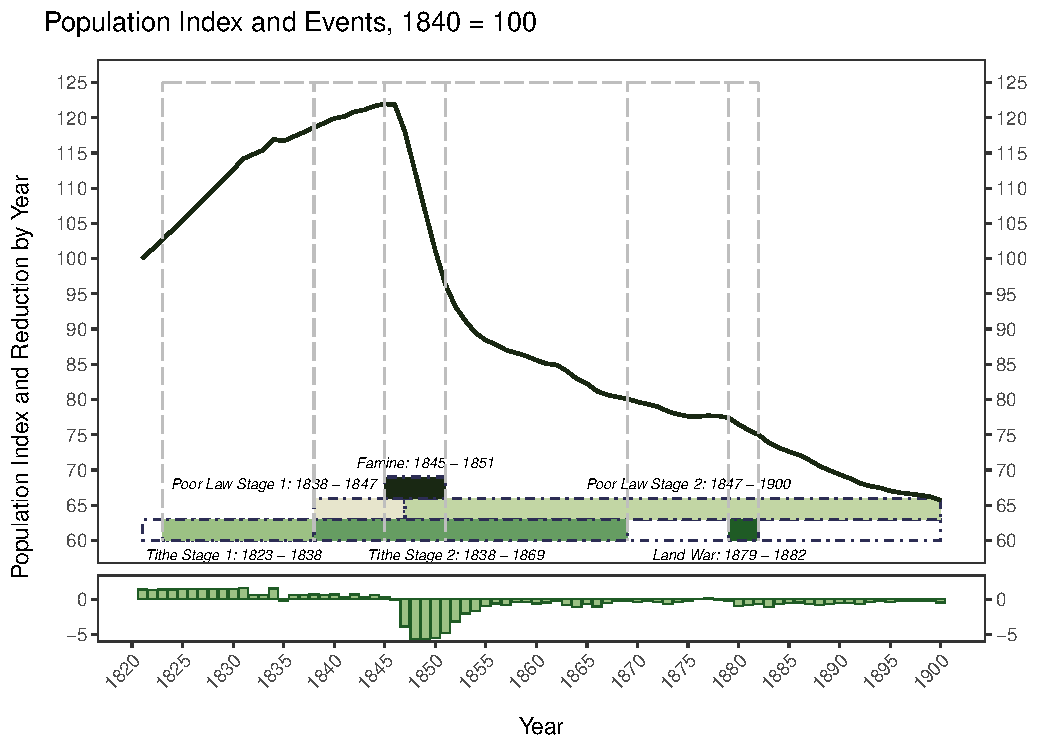
\includegraphics[width=.95\textwidth]{../03_outputs/popline.pdf}
\end{figure}

The first point in time when population growth slowed down was in 1838, when the reform of the tithe and poor laws took place; the second point was the period of famine, when the population began to decline significantly.

Figure 3.2 depicts the movement of cereal prices throughout the 19th century, especially during the famine, which helps us to visualize the subsequent regression model. When we correspond to the price curves and the population change curves in Figure 3.1, it appears we can see a link between peaks in price and peaks in population decline, for example, the peak in the price of potatoes and oats in 1879, coupled with the effects of the Land War, and the correspondingly rapid decline in population. While at 1882, the decline in population slowed down after the Land Wars, and also related to the relatively smoother society and prices.

\begin{figure}[htbp]
    \centering
    \caption{Grain Price, 1821 \textendash\ 1900}
    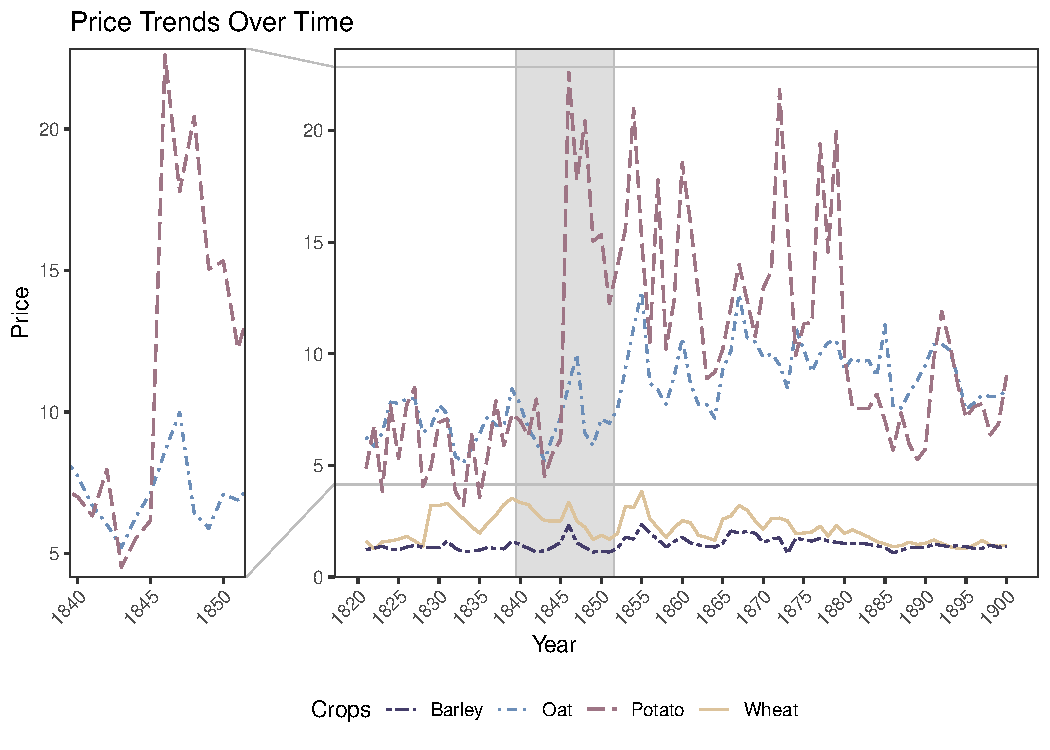
\includegraphics[width=.95\textwidth]{../03_outputs/grain_price.pdf}
\end{figure}

Also we must pay attention to theory of substitution. Potatoes and oats, as the dominant Irish crops of the 19th century and in the Irish diet, should have been substitutes for each other. The relationship between their prices can be seen in Figure 3.3.

\begin{figure}[htbp]
    \centering
    \caption{Potato Price \& Oat Price, 1821 \textendash\ 1900}
    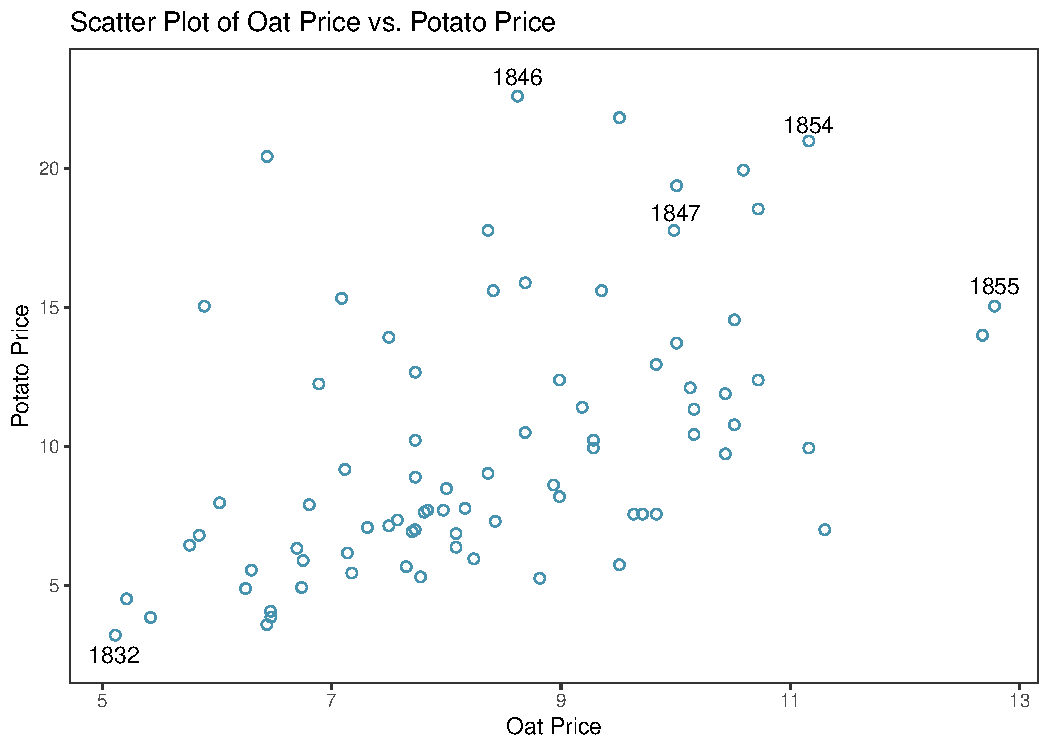
\includegraphics[width=.95\textwidth]{../03_outputs/grain_substituion.pdf}
\end{figure}

The arrows describe the price trends of the two grains during the famine, and the suddenly rise in the prices of both grains in 1846 may be directly related to the severe disaster of 1847, i.e., as stated earlier, an impairment of trade-based entitlement. While at the same time the sustained increase in the price of potatoes but the decrease in the price of the substitute oats from 1847 to 1848, as well as subsequent fluctuations in the prices of both, seem to foreshadow the famine and it was fading.

For Figure 3.3, there are two other noteworthy points in time, 1832 and 1855, where the coordinates for 1832 show that both potato and oat prices were at extremely low levels, corresponding to well-established farmers' trade-based entitlements, and historically, a period of rapid population growth in Ireland. But in 1855, when the famine had already passed, it can be noted that the price of oats in 1855 was abnormal, however, the fact that famine did not continue in 1855 was largely due to prices of other grains, including potatoes, wheat, barley, etc., did not rise in the same year, and the existence of substitutes compensated for the farmers' impaired trade-based entitlement.

Before proceeding with the regression, it is necessary to review the relationship between the variables. Figure 3.4 depicts the relationship between the independent variables and between the independent and dependent variables, where the gaps indicate insignificant correlation coefficients. The correlations between the independent variables are not repeated here because they are largely consistent with empirical inferences, e.g., the moderate correlation between potato prices and the prices of other cereals, the weak negative correlation between volume of imports and exports, etc. Also there is no high correlation between the independent variables.

\begin{figure}[htbp]
    \centering
    \caption{Regression Correlation Matrix}
    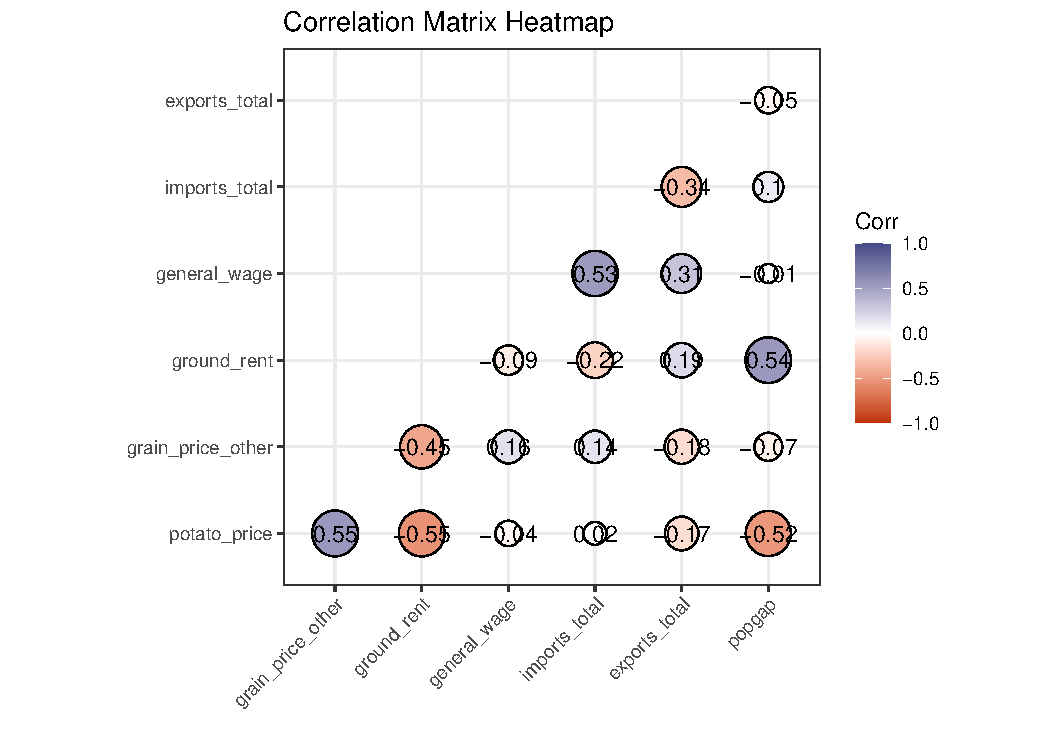
\includegraphics[width=.95\textwidth]{../03_outputs/corrmatrix.pdf}
\end{figure}

More noteworthy is the relationship between independent and dependent variables in Figure 3.4. The dependent variable \texttt{popgap} is significantly related  to \texttt{potato\_price}, \texttt{ground\_rent}, \texttt{grain\_acre\_total} and \texttt{imports\_total}. However, non-significant correlation coefficients do not directly lead to the conclusion that they should be excluded from the regression model \textemdash\ this tends to lead us to ignore non-linear relationship in nature. This paper will further explore these potential nonlinear relationships in the next chapter, along with a discussion of the regression methods used.

\section{Replication}

All the replication file can be found in this website:

\url{https://github.com/chxiii/Dissertation_Summer2024}

